\section{Metoda nierówności trójkąta}
Metoda nierówności trójkąta jest sposobem indeksowania danych optymalizującym wyznaczanie $ \varepsilon $-otoczenia. Działanie tej metody opiera się na wykorzystaniu nierówności trójkąta, dlatego bezpośrednie wykorzystanie metody nierówności trójkąta jest niemożliwe, jeśli korzystamy z miary, która nie spełnia nierówności trójkąta\footnote{W \cite{cosbyeuc} pokazano pośrednie wykorzystanie własności nierówności trójkąta do wyszukiwania $ \varepsilon $-otoczenia względem miary kosinusowej, która tej własności nie zachowuje. Rozwiązanie przedstawione w \cite{cosbyeuc} polega na sprowadzeniu wyznaczania $\varepsilon$-otoczenia względem miary kosinusowej, do wyznaczania $\varepsilon'$-otoczenia, gdzie $\varepsilon'$ jest deterministycznie zależne od $ \varepsilon $, względem miary euklidesowej, zachowującej własność nierówności trójkąta.}.
\subsection{Algorytm wyszukiwania $\varepsilon$-otoczenia}
Przedstawiany algorytm wyszukiwania $\varepsilon$-otoczenia jest oparty na propozycji \cite{tidbscan}. Zakładam, że dla dowolnych trzech punktów $ p $, $ q $ i $ r $ zachodzi \myhyperref{eq:ti-raw}{nierówność} względem miary odległości $ d $, czyli miary spełniającej następujące warunki:
\begin{equation} \label{eq:metric}
	\left\{\begin{array}{l}
		d(p,q)=0 \iff p=q \\
		d(p,q)=d(q,p) \\
		d(p,q)\leq d(p,r) + d(r,q) \;\;\;\;\text{// nierówność trójkąta}
	\end{array}\right.
\end{equation}
Jeśli wykorzystywana jest miara, która nie spełnia \myhyperref{eq:metric}{warunków} i w konsekwencji \myhyperref{eq:ti-raw}{nierówności}, to nie można bezpośrednio wykorzystać metody nierówności trójkąta.
\begin{equation}\label{eq:ti-raw}
	d(p,q) \ge \abs{d(p,r)-d(q,r)}
\end{equation}
Wartość $\abs{ d(p,r) - d(q,r) }$ będę dalej oznaczał $ d_r(p,q) $.
\begin{equation}\label{eq:ti}
	d(p,q) \ge d_r(p,q)
\end{equation}
 Punkt $ r $ będę nazywał punktem referencyjnym i zakładam, że jest dowolnie wybranym punktem, niekoniecznie należącym do zbioru danych $ D $. Punkty $ p $ i $ q $ należą do $ D $. \myhyperref{eq:ti}{Nierówność} można wykorzystać do wydajnego wyznaczenia $ \varepsilon $-otoczenia (\myhyperref{eq:eps-neighbourhood}{wyrażenie}) punktu $ p $. Jeśli wartość $ d_r(p,q) > \varepsilon $, to wiemy, że $ q $ nie należy do $ \varepsilon $-otoczenia punktu $ q $.
\begin{equation}
	d(p,q) \ge d_r(p,q) > \varepsilon \implies d(p,q) > \varepsilon \implies q \notin N_{D,\varepsilon}(p)
\end{equation}
Co więcej, jeśli $ q $ należy do $ \varepsilon $-otoczenia $ p $, to na pewno $ d_r(p,q) $ jest mniejsze lub równe $ \varepsilon $.
\begin{equation}
	q \in N_{D,\varepsilon}(p) \implies d(p,q) \le \varepsilon \implies d_r(p,q) \le \varepsilon
\end{equation}
Punktów należących do $ \varepsilon $-otoczenia punktu $ p $ należy zatem szukać pośród punktów spełniających warunek $ d_r(p,q) \le \varepsilon $, przy czym niekoniecznie wszystkie z tych punktów należą do $ \varepsilon $-otoczenia punktu $ p $, bo nie jest prawdą, że $ d_r(p,q) \le \varepsilon \implies q \in N_{D,\varepsilon}(p)$. Okazuje się, że można zapewnić szybki dostęp do punktów spełniających warunek $ d_r(p,q) \le \varepsilon $.
\begin{equation}\label{eq:ti-search-range}
	d_r(p,q) = \abs{d(p,r)-d(q,r)} \le \varepsilon \implies d(q,r) \in \left[d(p,r)-\varepsilon,d(p,r)+\varepsilon\right]
\end{equation}
\myhyperref{eq:ti-search-range}{Wyrażenie} pokazuje, że należy szukać punktów $ q $, dla których odległość od punktu referencyjnego znajduje się w przedziale $ \left[d(p,r)-\varepsilon,d(p,r)+\varepsilon\right]$. Jeśli stworzymy listę punktów należących do zbioru $ D $ posortowanych po odległości od punktu referencyjnego $ r $, to punkty należące do poszukiwanego zbioru $ \left[d(p,r)-\varepsilon,d(p,r)+\varepsilon\right] $ będą znajdowały się na pozycjach przed oraz po punkcie $ p $. Zaczynając w pozycji punktu $ p $, należy przesuwać się w przód listy i dla każdego kolejnego punktu $ q $ sprawdzać, czy należy do $ \varepsilon $-otoczenia punktu $ p $. Sprawdzanie kończymy, kiedy trafimy na punkt $ q $, dla którego $ d(q,r) $ nie mieści się w przedziale $ \left[d(p,r)-\varepsilon,d(p,r)+\varepsilon\right] $. Analogicznie postępujemy, przesuwając się w tył listy. Wynikiem jest $ \varepsilon $-otoczenie punktu $ p $, zawierające każdy ze sprawdzonych punktów, który spełnia warunek $ d(p,q) \le \varepsilon $ oraz punkt $ p $.
\begin{figure}
		\begin{minipage}[b]{.5\linewidth}
			\centering
			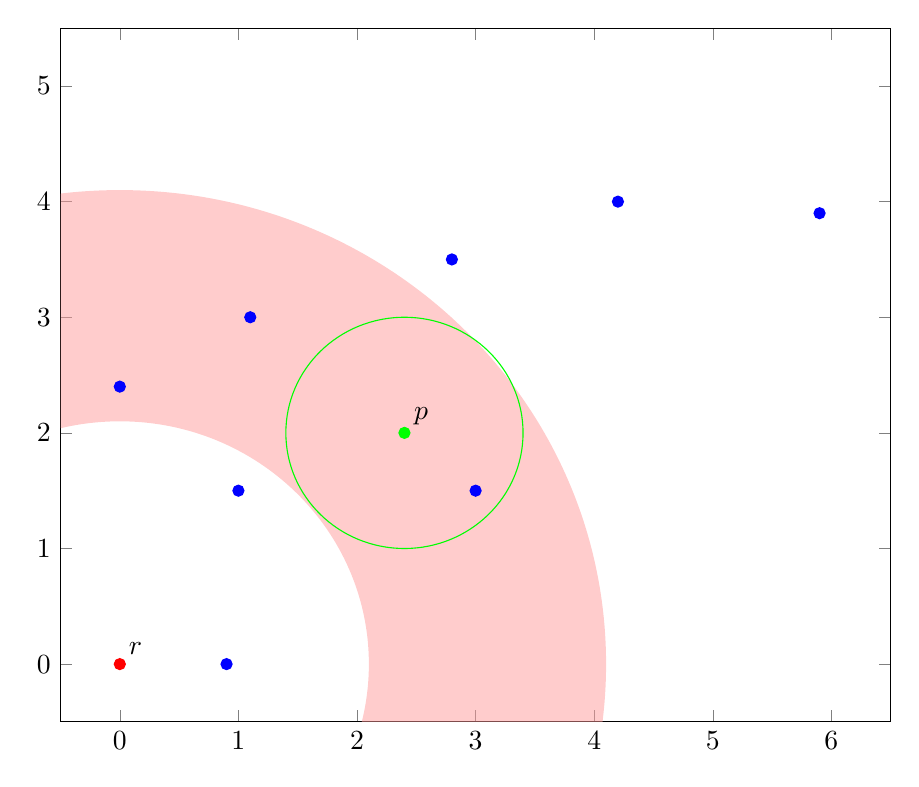
\begin{tikzpicture}[even odd rule]
			\begin{axis}[
			height=0.857\linewidth,
			width=\linewidth,
			xmin=-.5,ymin=-0.5,
			xmax=6.5,ymax=5.5
			]
	    
	    \fill[red!40, opacity=.5] (0,0) circle[radius=2.1] circle[radius=4.1];
			
			\addplot[blue, only marks] coordinates{ (0.9, 0) (1, 1.5) (0, 2.4) (1.1, 3) (3, 1.5) (2.8, 3.5) (4.2, 4) (5.9, 3.9)  };
			
			\addplot[green, mark=*, nodes near coords=$ p $,every node near coord/.style={black, anchor=225}, only marks] coordinates {(2.4, 2)};
			\draw[green] (2.4, 2) circle[radius=1];
			
			\addplot[red, mark=*, nodes near coords=$ r $,every node near coord/.style={black, anchor=225}, only marks] coordinates {(0,0)};
			    
			\end{axis}
			\end{tikzpicture}
		\end{minipage}%
		\begin{minipage}[b]{.5\linewidth}
			\centering
			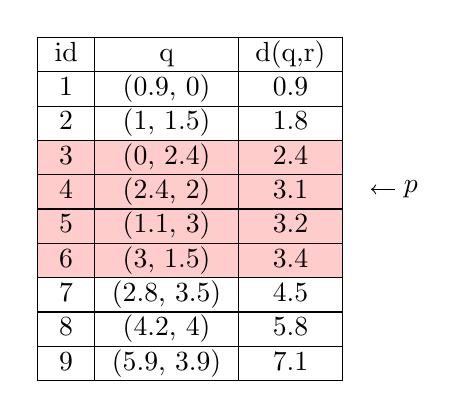
\begin{tikzpicture}
			 \node at (0,0) {\begin{tabular}{|c|c|c|}
			 	\hline 
			 	id& q & d(q,r) \\\hline
			 	1&(0.9, 0) & 0.9 \\\hline
			 	2&(1, 1.5) & 1.8 \\\hline
 	 			\rowcolor{red!20}
			 	3&(0, 2.4) & 2.4 \\\hline
 	 			\rowcolor{red!20}
			 	4&(2.4, 2) & 3.1 \\\hline
 	 			\rowcolor{red!20}
			 	5&(1.1, 3) & 3.2 \\\hline
 	 			\rowcolor{red!20}
			 	6&(3, 1.5) & 3.4 \\\hline
			 	7&(2.8, 3.5) & 4.5 \\\hline
			 	8&(4.2, 4) & 5.8 \\\hline
			 	9&(5.9, 3.9) & 7.1 \\\hline
			 	\end{tabular}};
			  \draw[<-] (2.3,.25) -- node[right=4pt] {$ p $} ++(.3,0); 
			\end{tikzpicture}
		\end{minipage}
		\caption{Wyznaczanie $ \varepsilon $-otoczenia punktu $ p=(2.4,2) $ metodą nierówności trójkąta dla punktu referencyjnego $ r=(0,0) $ i $ \varepsilon = 1$. Czerwonym kolorem oznaczono obszar, w którym odległość od punktu referencyjnego znajduje się w przedziale $ \left[d(p,r)-\varepsilon,d(p,r)+\varepsilon\right] $. Zielonym okręgiem oznaczono $ \varepsilon $-otoczenie punktu $ p $. Odległość od punktu $ p $ jest wyznaczana dla punktów 3,4,5,6. Punkty 4,6 tworzą $ \varepsilon $-otoczenia \mbox{punktu $ p $.}} \label{img:ti}
\end{figure}

Kompletną metodę nierówności trójkąta przedstawia \myhyperref{alg:ti}{algorytm}. Wdrożenie metody nierówności trójkąta do algorytmu DBSCAN ogranicza się do wyboru odpowiedniego $ r $ i wykonaniu następującego przypisania \linebreak\mbox{$ N_{D,\varepsilon}(p) \gets tineighbourhood(D, \varepsilon, r, p) $.}

\begin{algorithm}[t]
	\caption{Metoda nierówności trójkąta}\label{alg:ti}
	
	\DontPrintSemicolon
	
	\SetKwFunction{tineighbourhood}{tineighbourhood}
	
	\setcounter{AlgoLine}{0}
	\nonl\SetKwProg{myproc}{Wejście}{}{}
	\myproc{}{
		$ D $ - zbiór danych \;
		$\varepsilon $ - promień otoczenia \;
		$ r $ - punkt referencyjny \;
		$ p $ - punkt, dla którego jest wyznaczane $ \varepsilon $-otoczenie \;
	}
	\setcounter{AlgoLine}{0}
	\nonl\SetKwProg{myproc}{Wyjście}{}{}
	\myproc{}{
		$ \varepsilon $-otoczenie punktu $ p $\;
	}
	
	\setcounter{AlgoLine}{0}
	\nonl\SetKwProg{myproc}{Definicje}{}{}
	\myproc{}{
		$ sortid(p) $ - pozycja punktu $ p $ w zbiorze $ D $ posortowanym według odległości od $ r $\;
		$ at(i) $ - punkt na pozycji $ i $ w zbiorze $ D $ posortowanym według odległości od $ r $\;
	}
	\nonl\SetKwProg{myalg}{Algorytm}{}{}
	\myalg{\tineighbourhood{$D$, $\varepsilon$, $ r $, $ p $}}{
		$ N \gets \set{p}$\;
		$ i \gets sortid(p) - 1$\;
		\While{$ i \ge 1 \land d(at(i), r) \in \left[d(p,r)-\varepsilon,d(p,r)+\varepsilon\right]$}{
			\lIf{$ d(at(i),p) \le \varepsilon $}{$ N \gets N \cup {at(i)} $}
			$ i \gets i - 1 $\;
		}	
		\While{$ i \le |D| \land d(at(i), r) \in \left[d(p,r)-\varepsilon,d(p,r)+\varepsilon\right]$}{
			\lIf{$ d(at(i),p) \le \varepsilon $}{$ N \gets N \cup {at(i)} $}
			$ i \gets i + 1 $\;
		}		
		\KwRet{$ N $}
	}
\end{algorithm}

\subsection{Wydajność}
Szukamy $ \varepsilon $-otoczenia punktu $ p $ w zbiorze danych $ D $. Aby zapewnić efektywne działanie \myhyperref{alg:ti}{algorytmu} warto jest wcześniej wyznaczyć odległości dla każdego punktu $ q $ w zbiorze danych $ D $ od punktu referencyjnego $ r $ i odpowiednio posortować punkty zbioru danych $ D $ względem odległości od $ r $. W ten sposób możemy zapewnić stałą złożoność operacji $ sortid(p) $, $ at(i) $ oraz $ d(at(i), r) $ dla $ i \in \set{1,\dots,|D|} $. Jeśli te warunki zostaną spełnione, to możemy przyjąć, że najbardziej czasochłonną operacją \myhyperref{alg:ti}{algorytmu} jest wyznaczanie odległości między punktem $ p $, a punktami $ q $ należącymi do zbioru \mbox{$ R = \set{q | d(q, r) \in \left[d(p,r)-\varepsilon,d(p,r)+\varepsilon\right]} $}. 

Jeśli za operację podstawową uznamy obliczanie odległości, to złożoność obliczeniowa wyznaczania $ \varepsilon $-otoczenia za pomocą metody nierówności trójkąta zależy ściśle od liczebności zbioru $ R $. W pesymistycznym przypadku, dla dostatecznie dużej wartości $ \varepsilon $ liczebność $ R $ może równać się liczebności $ D $. Jeśli założyć, że odwzorowanie zbioru $ D $ na zbiór odległości od punktu referencyjnego $ T $ posiada rozkład równomierny, to liczebność zbioru $ R $ można przybliżyć jako stosunek $ \frac{2\varepsilon}{\max(T)-\min(T)} $. 

Wydajność metody nierówności trójkąta można poprawić, zmniejszając wartość $ \varepsilon $. Wartość $ \varepsilon $ jest jednak parametrem, od którego zależy rezultat algorytmu i nie można go swobodnie zmieniać bez wpływu na wynik. Można za to wpływać na wartość $ m=\max(T)-\min(T) $ bez wpływu na otrzymywane $ \varepsilon $-otoczenie. Wartość $ m $ zależy od doboru punktu referencyjnego $ r $. Można przyjąć, że powinno się tak dobierać $ r $, żeby maksymalizować wartość $ m $. 

\subsubsection{Wybór punktu referencyjnego}
Wybór punktu referencyjnego  $ r $ jest decydujący dla wydajności metody nierówności trójkąta. Pierwszą zasadą, jaką powinno się kierować przy wyborze punktu referencyjnego, jest wybieranie punktu, który jest wystarczająco odległy od zbioru danych. Dobrym wyborem są zwykle punkty znajdujące się poza zakresem wartości punktów zbioru danych. $ \myhyperref{img:ti-by-ref}{Rysunek} $ przedstawia dwa warianty wyboru punktu referencyjnego. Na $ \myhyperref{img:ti-by-ref-bad}{rysunku} $ został wybrany punkt niezgodny z zaleceniami, znajdujący się pośród punktów zbioru danych. Wyraźnie widać, że na $ \myhyperref{img:ti-by-ref-bad}{rysunku} $ wyznaczenie $ \varepsilon $-otoczenia punktu $ p $ wymaga wyznaczenia odległości od większej liczby punktów niż na $ \myhyperref{img:ti-by-ref-good}{rysunku} $.

\begin{figure}
	\begin{minipage}[b]{.5\linewidth}
		\centering
		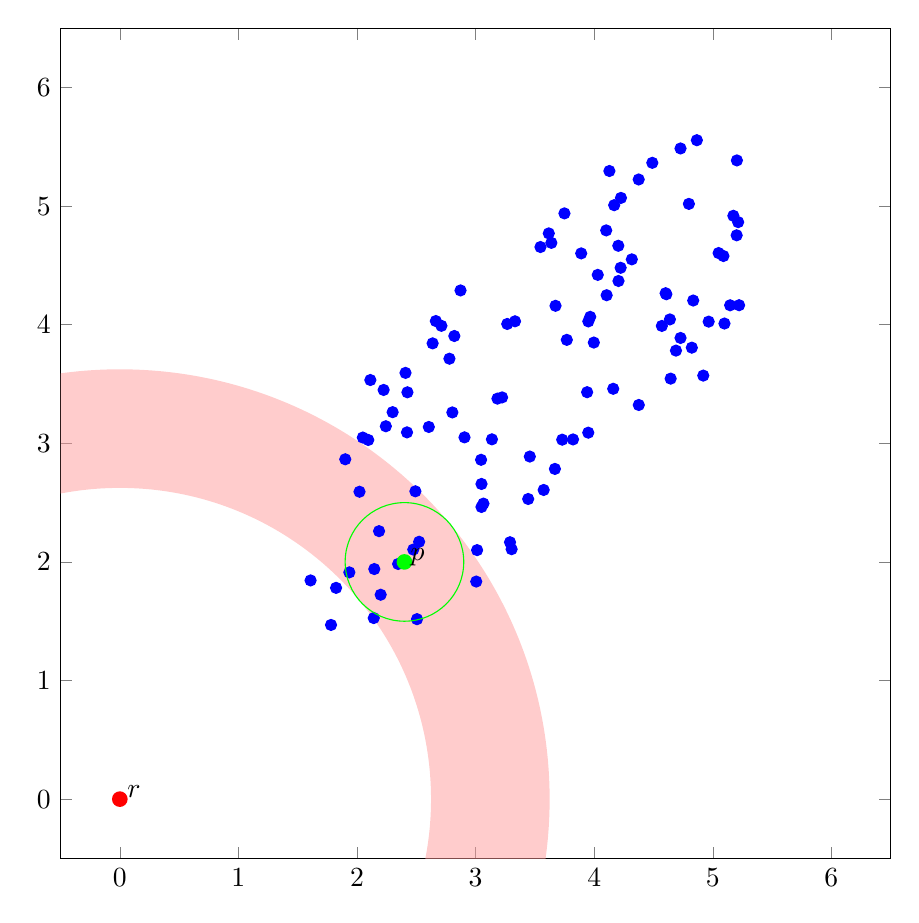
\begin{tikzpicture}[even odd rule]
		\begin{axis}[
		height=\linewidth,
		width=\linewidth,
		xmin=-.5,ymin=-.5,
		xmax=6.5,ymax=6.5, 
		clip marker paths=true
		]
		
		\def\eps{.5}
		\def\Rx{0}\def\Ry{0}
		\def\Px{2.4}\def\Py{2}
		\coordinate (R) at (\Rx,\Ry);
		\coordinate (P) at (\Px,\Py);
		\def\d{sqrt((\Rx-\Px)^2+(\Ry-\Py)^2)};
		
		\fill[red!40, opacity=.5] (R) circle[radius=\d-\eps] circle[radius=\d+\eps];
		
		\addplot[blue, only marks] coordinates{ (2.1995,1.7233) (5.0489,4.6042) (2.0210,2.5917) (3.7690,3.8723) (4.8231,3.8066) (3.4570,2.8884) (4.2046,4.3688) (2.0490,3.0487) (3.0496,2.6573) (3.8215,3.0328) (5.2011,4.7540) (3.9499,3.0897) (5.1460,4.1639) (5.2137,4.8651) (1.6085,1.8440) (3.9403,3.4311) (3.9662,4.0663) (3.6169,4.7701) (2.2244,3.4501) (4.7983,5.0188) (2.4089,3.5939) (3.0126,2.0995) (3.2667,4.0064) (4.4899,5.3650) (4.8347,4.2040) (3.0660,2.4916) (4.6020,4.2656) (3.6737,4.1595) (4.7279,3.8884) (3.9504,4.0279) (2.6375,3.8428) (4.0299,4.4202) (5.1733,4.9184) (3.0495,2.4635) (3.6686,2.7841) (3.2232,3.3872) (2.5237,2.1697) (2.3466,1.9828) (3.9967,3.8496) (1.9354,1.9119) (1.7809,1.4686) (4.5704,3.9898) (3.0053,1.8344) (4.2255,5.0692) (3.5468,4.6551) (3.8903,4.6014) (4.9650,4.0260) (2.9063,3.0502) (1.9009,2.8654) (4.3759,3.3232) (2.4922,2.5953) (4.6893,3.7818) (5.2031,5.3853) (4.1011,4.7952) (2.8039,3.2605) (4.7277,5.4862) (4.9196,3.5711) (3.3037,2.1075) (3.3323,4.0288) (5.2217,4.1645) (2.0948,3.0283) (2.1858,2.2595) (2.7793,3.7134) (2.3003,3.2627) (2.1126,3.5337) (3.5739,2.6067) (2.1411,1.5267) (3.1841,3.3768) (3.1375,3.0336) (2.7116,3.9907) (5.0982,4.0099) (2.2430,3.1439) (2.4745,2.1041) (3.4433,2.5306) (1.8235,1.7812) (2.6055,3.1379) (4.8655,5.5557) (3.0461,2.8610) (4.3751,5.2246) (2.8728,4.2891) (4.6381,4.0447) (2.4215,3.0923) (4.1603,3.4598) (2.4251,3.4302) (4.1049,4.2487) (3.2901,2.1660) (4.6083,4.2569) (2.6646,4.0310) (3.7303,3.0307) (2.1458,1.9399) (4.1684,5.0080) (4.6445,3.5454) (5.0895,4.5793) (3.7489,4.9387) (2.8207,3.9049) (3.6387,4.6902) (4.1280,5.2961) (4.2032,4.6657) (4.3171,4.5511) (2.5058,1.5174) (4.2228,4.4800)  };
		
		\draw[green] (P) circle[radius=.5];
		\node[green,label={[label distance=-8pt]75:{$ p $}},circle,fill,inner sep=2pt] at (P) {};
		
		\node[red,label={[label distance=-6pt]75:{$ r $}},circle,fill,inner sep=2pt] at (R) {};
		
		\end{axis}
		\end{tikzpicture}
		\subcaption{}\label{img:ti-by-ref-good}
	\end{minipage}%
	\begin{minipage}[b]{.5\linewidth}
		\centering
		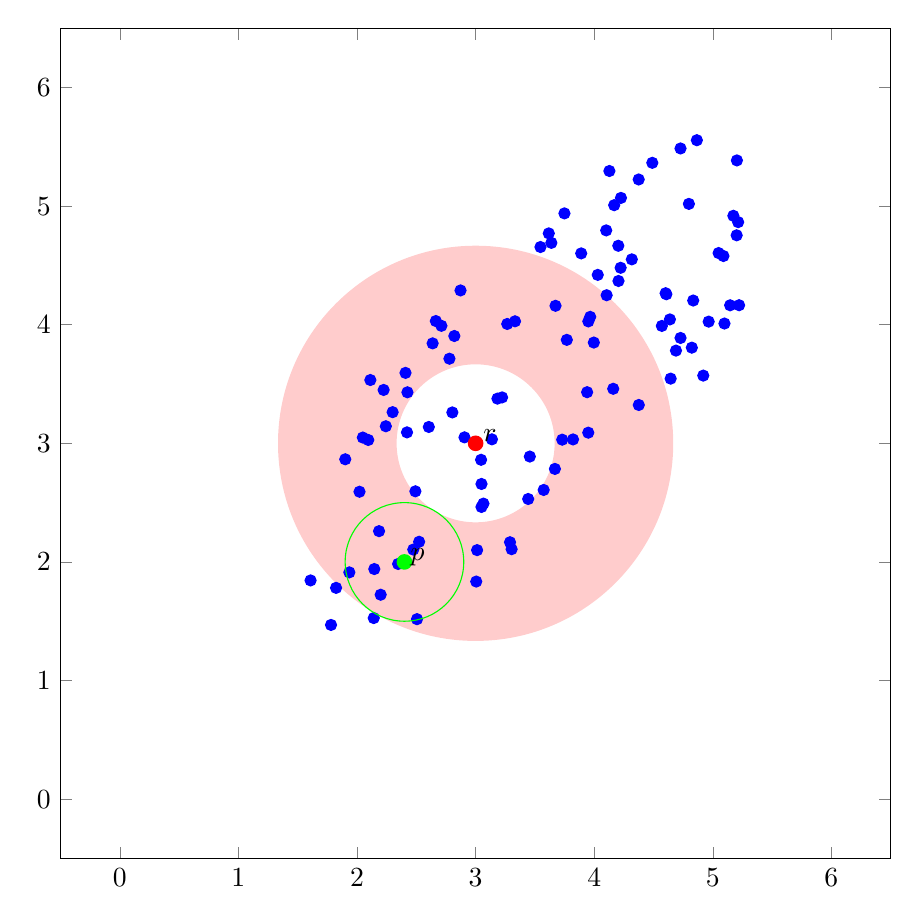
\begin{tikzpicture}[even odd rule]
		\begin{axis}[
		height=\linewidth,
		width=\linewidth,
		xmin=-.5,ymin=-.5,
		xmax=6.5,ymax=6.5, 
		clip marker paths=true
		]
		
		\def\eps{.5}
		\def\Rx{3}\def\Ry{3}
		\def\Px{2.4}\def\Py{2}
		\coordinate (R) at (\Rx,\Ry);
		\coordinate (P) at (\Px,\Py);
		\def\d{sqrt((\Rx-\Px)^2+(\Ry-\Py)^2)};
		
		\fill[red!40, opacity=.5] (R) circle[radius=\d-\eps] circle[radius=\d+\eps];
		
		\addplot[blue, only marks] coordinates{ (2.1995,1.7233) (5.0489,4.6042) (2.0210,2.5917) (3.7690,3.8723) (4.8231,3.8066) (3.4570,2.8884) (4.2046,4.3688) (2.0490,3.0487) (3.0496,2.6573) (3.8215,3.0328) (5.2011,4.7540) (3.9499,3.0897) (5.1460,4.1639) (5.2137,4.8651) (1.6085,1.8440) (3.9403,3.4311) (3.9662,4.0663) (3.6169,4.7701) (2.2244,3.4501) (4.7983,5.0188) (2.4089,3.5939) (3.0126,2.0995) (3.2667,4.0064) (4.4899,5.3650) (4.8347,4.2040) (3.0660,2.4916) (4.6020,4.2656) (3.6737,4.1595) (4.7279,3.8884) (3.9504,4.0279) (2.6375,3.8428) (4.0299,4.4202) (5.1733,4.9184) (3.0495,2.4635) (3.6686,2.7841) (3.2232,3.3872) (2.5237,2.1697) (2.3466,1.9828) (3.9967,3.8496) (1.9354,1.9119) (1.7809,1.4686) (4.5704,3.9898) (3.0053,1.8344) (4.2255,5.0692) (3.5468,4.6551) (3.8903,4.6014) (4.9650,4.0260) (2.9063,3.0502) (1.9009,2.8654) (4.3759,3.3232) (2.4922,2.5953) (4.6893,3.7818) (5.2031,5.3853) (4.1011,4.7952) (2.8039,3.2605) (4.7277,5.4862) (4.9196,3.5711) (3.3037,2.1075) (3.3323,4.0288) (5.2217,4.1645) (2.0948,3.0283) (2.1858,2.2595) (2.7793,3.7134) (2.3003,3.2627) (2.1126,3.5337) (3.5739,2.6067) (2.1411,1.5267) (3.1841,3.3768) (3.1375,3.0336) (2.7116,3.9907) (5.0982,4.0099) (2.2430,3.1439) (2.4745,2.1041) (3.4433,2.5306) (1.8235,1.7812) (2.6055,3.1379) (4.8655,5.5557) (3.0461,2.8610) (4.3751,5.2246) (2.8728,4.2891) (4.6381,4.0447) (2.4215,3.0923) (4.1603,3.4598) (2.4251,3.4302) (4.1049,4.2487) (3.2901,2.1660) (4.6083,4.2569) (2.6646,4.0310) (3.7303,3.0307) (2.1458,1.9399) (4.1684,5.0080) (4.6445,3.5454) (5.0895,4.5793) (3.7489,4.9387) (2.8207,3.9049) (3.6387,4.6902) (4.1280,5.2961) (4.2032,4.6657) (4.3171,4.5511) (2.5058,1.5174) (4.2228,4.4800)  };
		
		\draw[green] (P) circle[radius=.5];
		\node[green,label={[label distance=-8pt]75:{$ p $}},circle,fill,inner sep=2pt] at (P) {};
		
		\node[red,label={[label distance=-6pt]75:{$ r $}},circle,fill,inner sep=2pt] at (R) {};
		
		\end{axis}
		\end{tikzpicture}
		\subcaption{}\label{img:ti-by-ref-bad}
	\end{minipage}
	\caption{Wyznaczanie $ \varepsilon $-otoczenia punktu $ p $ dla $ \varepsilon=0.5 $ i różnych wariantów wyboru punktu referencyjnego $ r $. Punkty znajdujące się w czerwonym obszarze wymagają wyznaczenia odległości od $ p $.}\label{img:ti-by-ref}
\end{figure}
\begin{figure}
	\begin{minipage}[b]{.5\linewidth}
		\centering
		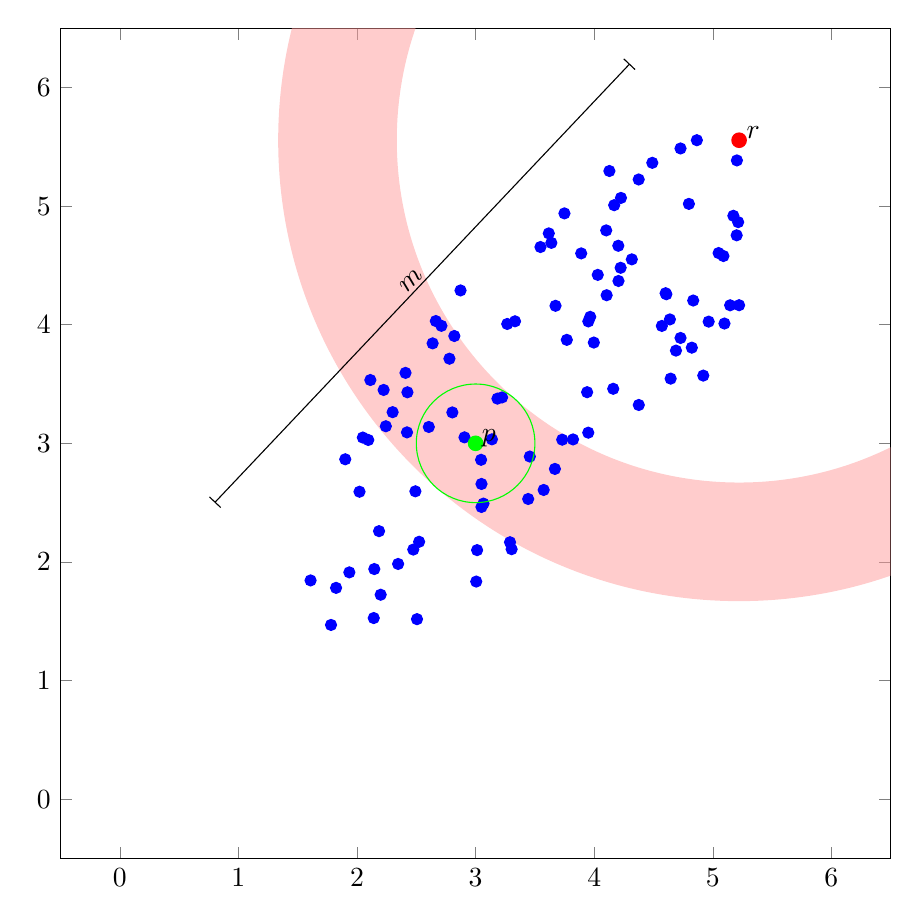
\begin{tikzpicture}[even odd rule]
		\begin{axis}[
		height=\linewidth,
		width=\linewidth,
		xmin=-.5,ymin=-.5,
		xmax=6.5,ymax=6.5, 
		clip marker paths=true
		]
		
		\def\eps{.5}
		\def\Rx{5.2217}\def\Ry{5.5557}
		\def\Px{3}\def\Py{3}
		\coordinate (R) at (\Rx,\Ry);
		\coordinate (P) at (\Px,\Py);
		\def\d{sqrt((\Rx-\Px)^2+(\Ry-\Py)^2)};
		
		\fill[red!40, opacity=.5] (R) circle[radius=\d-\eps] circle[radius=\d+\eps];
		
		\addplot[blue, only marks] coordinates{ (2.1995,1.7233) (5.0489,4.6042) (2.0210,2.5917) (3.7690,3.8723) (4.8231,3.8066) (3.4570,2.8884) (4.2046,4.3688) (2.0490,3.0487) (3.0496,2.6573) (3.8215,3.0328) (5.2011,4.7540) (3.9499,3.0897) (5.1460,4.1639) (5.2137,4.8651) (1.6085,1.8440) (3.9403,3.4311) (3.9662,4.0663) (3.6169,4.7701) (2.2244,3.4501) (4.7983,5.0188) (2.4089,3.5939) (3.0126,2.0995) (3.2667,4.0064) (4.4899,5.3650) (4.8347,4.2040) (3.0660,2.4916) (4.6020,4.2656) (3.6737,4.1595) (4.7279,3.8884) (3.9504,4.0279) (2.6375,3.8428) (4.0299,4.4202) (5.1733,4.9184) (3.0495,2.4635) (3.6686,2.7841) (3.2232,3.3872) (2.5237,2.1697) (2.3466,1.9828) (3.9967,3.8496) (1.9354,1.9119) (1.7809,1.4686) (4.5704,3.9898) (3.0053,1.8344) (4.2255,5.0692) (3.5468,4.6551) (3.8903,4.6014) (4.9650,4.0260) (2.9063,3.0502) (1.9009,2.8654) (4.3759,3.3232) (2.4922,2.5953) (4.6893,3.7818) (5.2031,5.3853) (4.1011,4.7952) (2.8039,3.2605) (4.7277,5.4862) (4.9196,3.5711) (3.3037,2.1075) (3.3323,4.0288) (5.2217,4.1645) (2.0948,3.0283) (2.1858,2.2595) (2.7793,3.7134) (2.3003,3.2627) (2.1126,3.5337) (3.5739,2.6067) (2.1411,1.5267) (3.1841,3.3768) (3.1375,3.0336) (2.7116,3.9907) (5.0982,4.0099) (2.2430,3.1439) (2.4745,2.1041) (3.4433,2.5306) (1.8235,1.7812) (2.6055,3.1379) (4.8655,5.5557) (3.0461,2.8610) (4.3751,5.2246) (2.8728,4.2891) (4.6381,4.0447) (2.4215,3.0923) (4.1603,3.4598) (2.4251,3.4302) (4.1049,4.2487) (3.2901,2.1660) (4.6083,4.2569) (2.6646,4.0310) (3.7303,3.0307) (2.1458,1.9399) (4.1684,5.0080) (4.6445,3.5454) (5.0895,4.5793) (3.7489,4.9387) (2.8207,3.9049) (3.6387,4.6902) (4.1280,5.2961) (4.2032,4.6657) (4.3171,4.5511) (2.5058,1.5174) (4.2228,4.4800)  };
		
		\draw[green] (P) circle[radius=.5];
		\node[green,label={[label distance=-8pt]75:{$ p $}},circle,fill,inner sep=2pt] at (P) {};
		
		\node[red,label={[label distance=-6pt]75:{$ r $}},circle,fill,inner sep=2pt] at (R) {};
		
		\draw[|-|] (.8,2.5) -- node[above=-3pt,rotate=45]{$ m $} +(3,3.2);
		
		\end{axis}
		\end{tikzpicture}
		\subcaption{}\label{img:ti-max-ref-good}
	\end{minipage}%
	\begin{minipage}[b]{.5\linewidth}
		\centering
		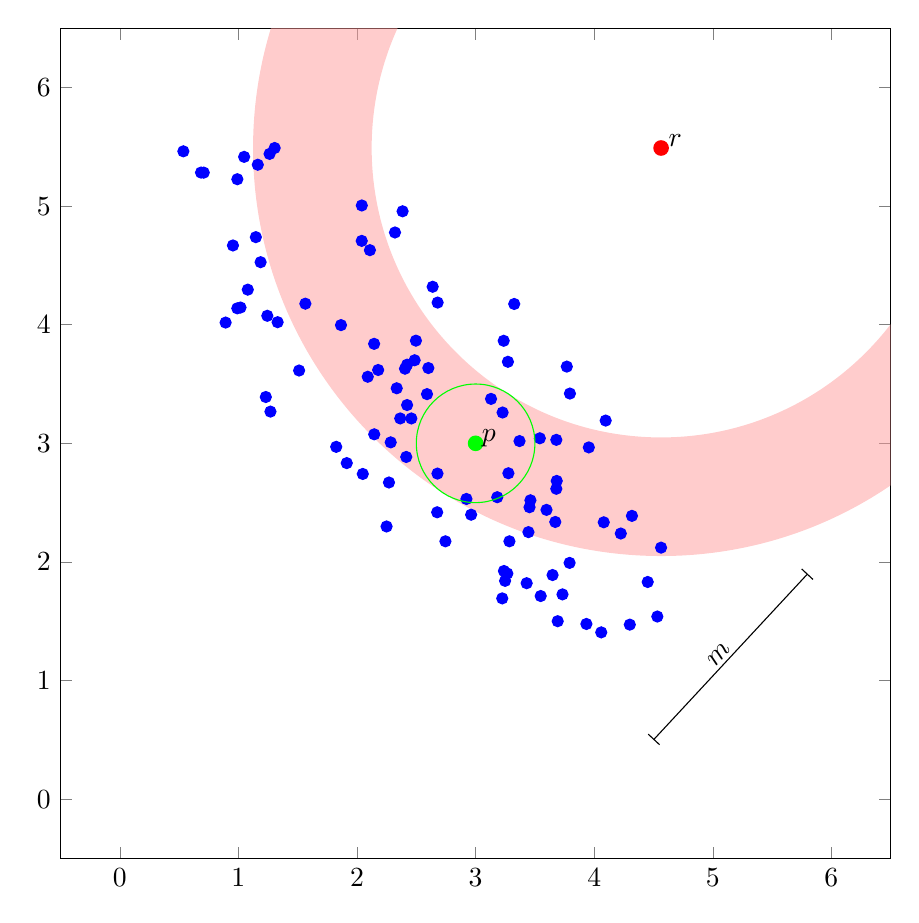
\begin{tikzpicture}[even odd rule]
		\begin{axis}[
		height=\linewidth,
		width=\linewidth,
		xmin=-.5,ymin=-.5,
		xmax=6.5,ymax=6.5, 
		clip marker paths=true
		]
		
		\def\eps{.5}
		\def\Rx{4.5638}\def\Ry{5.4900}
		\def\Px{3}\def\Py{3}
		\coordinate (R) at (\Rx,\Ry);
		\coordinate (P) at (\Px,\Py);
		\def\d{sqrt((\Rx-\Px)^2+(\Ry-\Py)^2)};
		
		\fill[red!40, opacity=.5] (R) circle[radius=\d-\eps] circle[radius=\d+\eps];
		
		\addplot[blue, only marks] coordinates{ (2.38440,4.95645) (1.82466,2.97027) (3.27246,3.68736) (2.74550,2.17377) (3.28522,2.17373) (2.41511,2.88507) (0.89206,4.01807) (3.76900,3.64688) (3.22459,1.69251) (1.91358,2.83324) (2.45815,3.20958) (1.27008,3.26737) (3.45469,2.46123) (1.16332,5.34880) (2.67591,2.41845) (4.22413,2.23948) (3.27639,2.74761) (3.54147,3.04247) (1.23111,3.39052) (3.69212,1.50015) (2.63786,4.32009) (3.23892,1.92352) (3.67175,2.33692) (2.59022,3.41486) (4.09670,3.19172) (1.24366,4.07522) (2.32016,4.77767) (2.03980,4.70684) (3.64886,1.88952) (2.67979,4.18666) (2.26942,2.66964) (2.10877,4.62868) (2.14531,3.07587) (0.70780,5.28235) (2.96227,2.39816) (3.23679,3.86448) (3.73255,1.72628) (4.31822,2.38824) (3.79525,3.41967) (1.04828,5.41530) (2.04868,2.74172) (1.18715,4.52725) (2.24923,2.29874) (2.36440,3.20979) (2.67840,2.74469) (2.60147,3.63476) (2.09054,3.56112) (3.68402,2.68288) (3.13007,3.37461) (3.24850,1.84035) (3.68045,2.61670) (2.17830,3.61835) (2.14424,3.83881) (2.40479,3.62923) (1.51182,3.61380) (0.68485,5.28291) (3.59778,2.43879) (3.54870,1.71243) (3.44547,2.25123) (3.26748,1.90228) (1.33064,4.02150) (1.30563,5.48999) (1.07900,4.29560) (2.42236,3.32276) (1.56454,4.17744) (2.04039,5.00547) (3.46219,2.51972) (4.53221,1.53949) (3.32553,4.17491) (3.43039,1.82064) (2.28417,3.00811) (3.37019,3.01888) (2.92268,2.53094) (3.95454,2.96549) (3.22761,3.25976) (0.99102,5.22679) (2.33482,3.46416) (0.99058,4.13824) (2.49679,3.86558) (2.48593,3.70032) (3.79252,1.99178) (1.14713,4.73841) (4.08042,2.33411) (4.45110,1.83085) (4.05931,1.40595) (3.93414,1.47682) (0.53578,5.46202) (4.30019,1.47117) (1.86496,3.99669) (4.56378,2.12047) (3.18252,2.54561) (1.26280,5.44026) (1.01758,4.14484) (0.95393,4.66833) (3.68063,3.02927) (2.42245,3.66298) };
		
		\draw[green] (P) circle[radius=.5];
		\node[green,label={[label distance=-8pt]75:{$ p $}},circle,fill,inner sep=2pt] at (P) {};
		
		\node[red,label={[label distance=-6pt]75:{$ r $}},circle,fill,inner sep=2pt] at (R) {};
		
		\draw[|-|] (4.5,.5) -- node[above=-3pt,rotate=48]{$ m $} +(.8,.9);
		
		\end{axis}
		\end{tikzpicture}
		\subcaption{}\label{img:ti-max-ref-bad}
	\end{minipage}
	\caption{Wyznaczanie $ \varepsilon $-otoczenia \mbox{punktu $ p $} dla $ \varepsilon =0.5 $ i różnych wariantów rozkładu danych. Punkt referencyjny $ r $ został wybrany zgodnie z \myhyperref{eq:ti-max-ref}{wyrażeniem}. Punkty znajdujące się w czerwonym obszarze wymagają wyznaczenia odległości od $ p $.}\label{img:ti-max-ref}
\end{figure}

Jednym ze sposobów na wybranie efektywnego punktu referencyjnego jest wybór takiego punktu, że wartość $i $-tej współrzędnej punktu $ r $ jest równa wartości maksymalnej(albo minimalnej) tej współrzędnej w \mbox{zbiorze $ D $.}
\begin{equation}\label{eq:ti-max-ref}
	r=(a_1,\dots,a_{dim(D)})\ :\ a_i = max(\set{b_i | (b_1,\dots,b_{dim(D)}) \in D)})
\end{equation}
Niestety skuteczność tej metody jest wrażliwa na rozkład punktów w zbiorze danych. \myhyperref{img:ti-max-ref}{rysunki} przedstawiają sytuacje dla różnych rozkładów punktów. Na \myhyperref{img:ti-max-ref-good}{rysunku} położenie punktu $ r $ jest korzystniejsze i wartość $ m $ jest większa niż na \myhyperref{img:ti-max-ref-bad}{rysunku}. W pewnym stopniu można sobie z tym problemem poradzić, wyznaczając punkty referencyjne dla różnych kombinacji minimum lub maksimum dla poszczególnych współrzędnych (np. $ r=(a_{1max}, a_{2min}, a_{3min}, \dots) $). Następnie, dla każdego z punktów referencyjnych można wyznaczyć $ m $ i wybrać $ r $, dla którego $ m $ jest największe. Wyznaczenie wartości $ m $ dla danego $ r $ jest realizowalne w czasie liniowym, ale wygenerowanych punktów referencyjnych może być $ 2^{dim(D)} $. Aby uniknąć problemów wydajnościowych w przypadku wysokowymiarowych danych, można się ograniczyć do $ k $ spośród wygenerowanych punktów referencyjnych. 

\begin{table}[h] 
	\footnotesize
	\tabcolsep=0.11cm
	\centering
	\begin{tabular}{|c|c|c|c|c|c|c|c|c|c|c|c|c|c|c|c|}
		\hline 
		$D$			&$ \varepsilon $ & $ \mu $ & $|D|$&$dim(D)$&$m$&$mad$&$sd$&$T_s [s]$&$T[s]$\\\hline
		sequoia&4000&4&62556&2&1.36e+06&2.82e+05&3.29e+05&0.08&0.57\\\hline
		sequoia&4000&4&62556&2&1.19e+06&7.75e+04&9.13e+04&0.08&1.71\\\hline
		birch&4000&4&100000&2&1.31e+06&2.16e+05&2.63e+05&0.13&1.50\\\hline
		birch&4000&4&100000&2&1.31e+06&2.17e+05&2.63e+05&0.13&1.49\\\hline
		cup98&40&4&96367&56&7900.55&843.33&1241.64&0.17&42.11\\\hline
		cup98&40&4&96367&56&8129.04&868.62&1270.16&0.17&36.27\\\hline
		covtype&120&4&50000&55&7024.42&1079.42&1362.62&0.09&11.47\\\hline
		covtype&120&4&50000&55&8462.06&1217.56&1547.69&0.08&9.77\\\hline
	\end{tabular}
	\caption{Grupowania zbioru danych $ D $ algorytmem DBSCAN z metodą nierówności trójkąta. $ mad $ - średnie bezwględne odchylenie odległości od punktu referencyjnego, $ sd $ - odchylenie standardowe odległości od punktu referencyjnego, $ T_s $ - czas sortowania, $ T $ - całkowity czas grupowania}\label{tbl:ti-time-by-ref}
\end{table}
Doświadczenia pokazują, że dobrymi wskaźnikami efektywności wybranego punktu referencyjnego, poza $ m $, mogą też być wartości odchylenia standardowego lub bezwzględnego średniego odchylenia odległości od punktu referencyjnego, przy czym należy te wartości maksymalizować. \myhyperref{tbl:ti-time-by-ref}{Tabela} przedstawia przykłady czasu grupowania rzeczywistych zbiorów danych w zależności od wartości wskaźników dla wybranego punktu referencyjnego.

\subsubsection{Wiele punktów referencyjnych}
Istnieje wariant metody nierówności trójkąta, który umożliwia wykorzystanie wielu punktów referencyjnych. Zakładam, że wyznaczane jest \linebreak$ \varepsilon $-otoczenie punktu $ p $ w zbiorze danych $ D $. Metoda nierówności trójkąta z wieloma punktami referencyjnymi działa podobnie jak zwykła metoda nierówności trójkąta. Nadal wymagane jest wybranie punktu referencyjnego $ r $, względem którego sortowany jest zbiór danych. Dodatkowo wybierany jest jeszcze zbiór innych punktów $ R $. Różnica w działaniu algorytmu polega na tym, że dodatkowo wprowadza się \myhyperref{eq:projection-mult}{warunek} na przynależność punktu $ q $ do $ \varepsilon $-otoczenia punktu $ p $.
\begin{equation}\label{eq:ti-reference-mult}
q \in N_{D,\varepsilon}(p) \implies  \forall_{\rho\in R}\,d(q,\rho) \in \left[d(p,\rho)-\varepsilon,d(p,\rho)+\varepsilon\right] 
\end{equation}
Dzięki wprowadzeniu \myhyperref{eq:projection-mult}{warunku} możemy uniknąć wyznaczania dystansu dla części punktów.

\begin{algorithm}[t]
	\caption{Metoda nierówności trójkąta z wieloma punktami referencyjnymi}\label{alg:ti-mult}
	
	\DontPrintSemicolon
	
	\SetKwFunction{multtineighbourhood}{multtineighbourhood}
	
	\setcounter{AlgoLine}{0}
	\nonl\SetKwProg{myproc}{Wejście}{}{}
	\myproc{}{
		$ D $ - zbiór danych \;
		$\varepsilon $ - promień otoczenia \;
		$ l $ - współrzędna projekcji \;
		$ R $ - zbiór dodatkowych punktów referencyjnych\;
		$ p $ - punkt, dla którego jest wyznaczane $ \varepsilon $-otoczenie \;
	}
	\setcounter{AlgoLine}{0}
	\nonl\SetKwProg{myproc}{Wyjście}{}{}
	\myproc{}{
		$ \varepsilon $-otoczenie punktu $ p $\;
	}
	
	\setcounter{AlgoLine}{0}
	\nonl\SetKwProg{myproc}{Definicje}{}{}
	\myproc{}{
		$ sortid(p) $ - pozycja punktu $ p $ w zbiorze $ D $ posortowanym według odległości od $ r $\;
		$ at(i) $ - punkt na pozycji $ i $ w zbiorze $ D $ posortowanym według odległości od $ r $\;
	}
	\nonl\SetKwProg{myalg}{Algorytm}{}{}
	\myalg{\multtineighbourhood{$D$, $\varepsilon$, $ r $, $ R $, $ p $}}{
		$ N \gets \set{p}$\;
		$ i \gets sortid(p) - 1$\;
		\While{$ i \ge 1 \land d(at(i), r) \in \left[d(p,r)-\varepsilon,d(p,r)+\varepsilon\right]$}{
			\If{$ \forall_{\rho\in R}\,d(at(i),\rho) \in \left[d(p,\rho)-\varepsilon,d(p,\rho)+\varepsilon\right] $}{
				\lIf{$ d(at(i),p) \le \varepsilon $}{$ N \gets N \cup {at(i)} $}
			}
			$ i \gets i - 1 $\;
		}	
		\While{$ i \le |D| \land d(at(i), r) \in \left[d(p,r)-\varepsilon,d(p,r)+\varepsilon\right]$}{
			\If{$ \forall_{\rho\in R}\,d(at(i),\rho) \in \left[d(p,\rho)-\varepsilon,d(p,\rho)+\varepsilon\right] $}{
				\lIf{$ d(at(i),p) \le \varepsilon $}{$ N \gets N \cup {at(i)} $}
			}
			$ i \gets i + 1 $\;
		}		
		\KwRet{$ N $}
	}
\end{algorithm} 